\documentclass[14pt]{article}
\usepackage[14pt]{extsizes}
\usepackage[utf8]{inputenc}
\usepackage[T2A]{fontenc}
\usepackage[russian, english]{babel}
\usepackage[a4paper,left=30mm, right=15mm, top=20mm, bottom=20mm]{geometry}
\usepackage{indentfirst, setspace}
\setlength{\parindent}{1.25cm}
\usepackage{tabularx, multirow}
\usepackage[normalem]{ulem}
\usepackage[style=russian]{csquotes}
\usepackage{graphicx,wrapfig}
\usepackage{amsmath,amsfonts,amssymb}
\usepackage{mathtools}
\usepackage{listings}
\usepackage{caption}
\usepackage{geometry}
\geometry{
	a4paper,
	left=30mm,
	right=15mm,
	top=20mm,
	bottom=20mm
}
\renewcommand{\labelenumii}{\arabic{enumi}.\arabic{enumii}.}
\renewcommand{\labelenumiii}{\arabic{enumi}.\arabic{enumii}.\arabic{enumiii}.}
\renewcommand{\labelenumiv}{\arabic{enumi}.\arabic{enumii}.\arabic{enumiii}.\arabic{enumiv}.}
\DeclareCaptionLabelSeparator{custom}{ --- }
\captionsetup{labelsep=custom}
\usepackage{pgfplots}
\usepackage{pdfpages}
\pgfplotsset{compat=1.9}
\usepackage{xcolor}
\usepackage{hyperref}
\definecolor{linkcolor}{HTML}{000000} 
\definecolor{urlcolor}{HTML}{000000} 
\hypersetup{pdfstartview=FitH,linkcolor=linkcolor,urlcolor=urlcolor, colorlinks=true}
\usepackage{tikz}
\usetikzlibrary{shapes.geometric, arrows}
\usetikzlibrary{positioning}
\usepackage{cmap}
\captionsetup[figure]{name=Рисунок}
\renewcommand{\lstlistingname}{Листинг}
\usepackage{cite}
\usepackage{listings}
\usepackage{listingsutf8}

\lstset{
	inputencoding=utf8,
	extendedchars=false,
	basicstyle=\ttfamily\small,
	breaklines=true,
	breakatwhitespace=true,
	showstringspaces=false,
	keepspaces=true,
	columns=fullflexible
}

\sloppy
\emergencystretch=3em


\begin{document}
	{\setstretch{1.0}
		\noindent
		\begin{tabular}{@{}m{0.18\textwidth}@{\hspace{0.02\textwidth}}m{0.8\textwidth}@{}}
			
\includegraphics[width=\linewidth]{1.png} &
			\centering
			\begin{bfseries}\small
				Министерство науки и высшего образования Российской Федерации\par
				Федеральное государственное\par
				автономное образовательное учреждение высшего образования\par
				\enquote{Московский государственный технический университет\par
					имени Н. Э. Баумана\par
					(национальный исследовательский университет)}\par
				(МГТУ им. Н. Э. Баумана)
			\end{bfseries}
		\end{tabular}
	}
	
	\vspace{0.5cm}
	
	{\setstretch{0.1}
		\noindent\rule{\textwidth}{1mm}
		\noindent\rule{\textwidth}{0.5mm}
		
	}
	
	\fontsize{14}{21}\selectfont
	
	\begin{tabularx}{\textwidth}{l >{\centering\arraybackslash}X}
		ФАКУЛЬТЕТ & \flqq Фундаментальные Науки\frqq \\ 
		
		КАФЕДРА & ФН-12 \flqq Математическое моделирование\frqq \\ 
	\end{tabularx}
	
	
	\vspace{1cm}
	
	
	\begin{center}
		\begin{bf}
			
			\fontsize{24}{36}\selectfont
			ОТЧЕТ
			
			\fontsize{20}{30}\selectfont
			ПО ЛАБОРАТОРНОЙ РАБОТЕ 
			
			\fontsize{20}{30}\selectfont
			по дисциплине <<Типы и структуры данных>>
			
			Тема: <<Сравнительный анализ рекурсивного и нерекурсивного алгоритмов>>
			
		\end{bf}
	\end{center}
	
	\fontsize{14}{21}\selectfont
	\vspace{5cm}
	
	
	\noindent\begin{tabularx}{\textwidth}{ X >{\centering}p{4cm} p{1cm} c }
		Выполнил студент группы ФН12-31Б: & & & Егоров К.Ю.\\ \cline{2-2} \cline{4-4}
		& \fontsize{10}{15}\selectfont дата, подпись & & \fontsize{10}{15}\selectfont Ф.И.О. \\
		Проверил преподаватель: & & & Строганов Ю.В.\\ \cline{2-2} \cline{4-4}
		& \fontsize{10}{15}\selectfont дата, подпись & & \fontsize{10}{15}\selectfont Ф.И.О.
		
	\end{tabularx}
	
	\vspace{\fill}
	
	\begin{center}
		\it{Москва}, 2025
	\end{center}
	
	\thispagestyle{empty}
	
	\newpage
	\renewcommand{\contentsname}{\centering{\foreignlanguage{russian}{СОДЕРЖАНИЕ}}}
	\setcounter{page}{2}
	\tableofcontents
	
	\newpage
	\begin{center}
		\section*{\foreignlanguage{russian}{ВВЕДЕНИЕ}} 
		\addcontentsline{toc}{section}{\foreignlanguage{russian}{ВВЕДЕНИЕ}}
	\end{center}
		
	Разработчики часто сталкиваются с дилеммой выбора между рекурсивными и итеративными подходами.\par
	\textbf{Цель работы}\par
	Провести сравнительный анализ рекурсивного и нерекурсивного алгоритмов.
	Для достижения поставленной цели требуется выполнить следующие задачи:\par
	1) разработать рекурсивный и нерекурсивный алгоритмы решения задачи, согласно варианту;\par
	2) описать средства разработки и инструменты замера процессорного времени выполнения реализации алгоритмов;\par
	3) реализовать разработанные алгоритмы;\par
	4) выполнить тестирование реализации алгоритмов;\par
	5) выполнить теоретическую оценку затрачиваемой реализацией каждого алгоритма памяти(для рекурсивного алгоритма --- на материале анализа высоты дерева рекурсивных вызовов и оценки затрачиваемой на один вызов функции памяти);\par
	6) выполнить замеры процессорного времени выполнения реализации алгоритмов в зависимости от варьируемого входа(одна точка на графике получается делением времени выполнения k идентичных расчетов на k, k >= 100);\par
	7) сделать выводы из сравнительного анализа реализации рекурсивного и нерекурсивного алгоритмов решения одной и той же задачи, заданной вариантом, по критериям ёмкостной эффективности(на материале теоретической оценки пиковой временной эффективности и на материале результатов измерений).
	\newpage
	\section{Аналитическая часть}
	\textbf{Рекурсивный алгоритм} --- это алгоритм, который решает задачу, вызывая сам себя один или несколько раз для решения тесно связанных подзадач. Эти вызовы называются рекурсивными вызовами [1].\par
	\textbf{Итеративный алгоритм} --- это алгоритм, который реализуется с помощью циклов(таких как for и while), которые повторяют выполнение блока операторов до достижения некоторого условия завершения. В отличие от рекурсии, итерация не требует организации стека вызовов и обычно более эффективна по использованию памяти [1].\par
	\textbf{Описание варианта для разработки алгоритмов}: Дана последовательность натуральных чисел(одно число в строке), завершающаяся числом 0. Выведите все нечетные числа из этой последовательности, сохраняя их порядок. В этой задаче нельзя использовать глобальные переменные и передавать какие-либо параметры в рекурсивную функцию. Функция получает данные, считывая их с клавиатуры. Функция не возвращает значение, а сразу же выводит результат на экран. Основная программа должна состоять только из вызова этой функции.
	\subsection{Вывод}
	Были приведены все основные термины и вариант для разработки алгоритмов.
	\newpage
	\section{Конструкторская часть}
	\subsection*{Блок-схема обоих алгоритмов}
	\begin{center}
		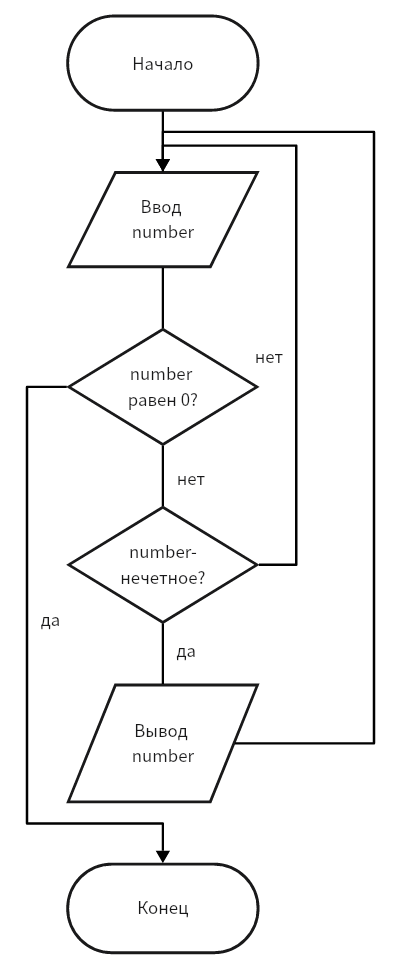
\includegraphics[width = 0.4\textwidth]{scheme.png}
	\end{center}
	\subsection{Вывод}
	Была приведена блок-схема, описывающая вариант, разработанный в виде итеративного алгоритма и рекурсивного алгоритма.
	\newpage
	\section{Технологическая часть} 
	\subsection{Выбор средств реализации}
	Для программной реализации поставленных задач использовалась среда разработки $Vi\-su\-al$ $Studio$ $Code$, используемый язык программирования — C++.
	Для компиляции кода использовался компилятор $g++$.
	Исследование проводилось на ноутбуке с такими техническими составляющими:\par
	1) оперативная память --- DDR4 16ГБ (скорость 3200 МТ/с);\par
	2) процессор --- 12th Gen Intel(R) Core(TM) i7-12700H (2.30 ГГц);\par
	3) тип системы --- 64-разрядная операционная система, процессор x64;\par
	5) операционная система --- Windows 11 Pro (сборка 26100.6584);\par
	6) диск --- SSD 954ГБ (NVMe).\par
	\subsection{Примеры работы программной реализации}
	\textbf{Использование первого режима}\par
	На рисунке~\ref{fig:1} представлен запуск программной реализации с такими входными данными для обоих алгоритмов: пять различных натуральных чисел с 0 в качестве шестого числа, среди которых будет два нечетных числа(на экране помимо введенных чисел должны быть продублированы нечетные числа).
	\begin{center}
		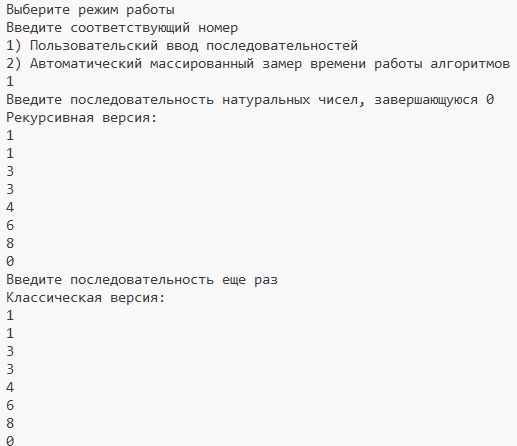
\includegraphics[width = 0.9\textwidth]{example_1.png}
		\captionof{figure}{Пример 1}
		\label{fig:1}
	\end{center}
	
	На рисунках~\ref{fig:2} и ~\ref{fig:3} представлены запуски программной реализации для обоих алгоритмов с такими входными данными: вводится некоторое количество натуральных чисел, после чего вводится отрицательное число(в этом случае программа должна выдать ошибку).
	\begin{center}
		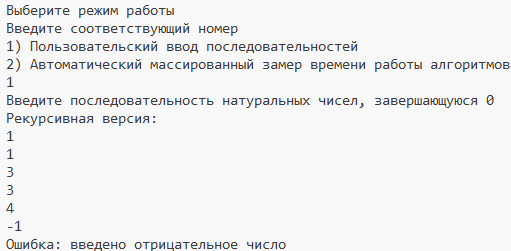
\includegraphics{example_2.png}
		\captionof{figure}{Пример 2}
		\label{fig:2}
	\end{center}
	\begin{center}
		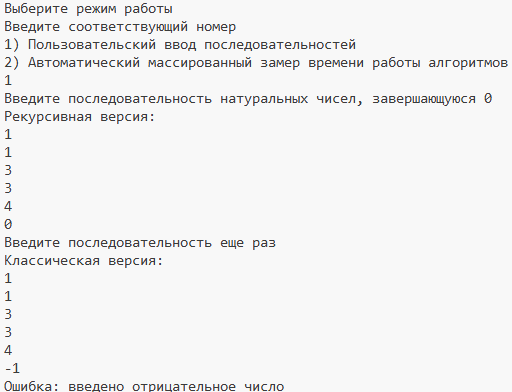
\includegraphics{example_3.png}
		\captionof{figure}{Пример 3}
		\label{fig:3}
	\end{center}
	\textbf{Использование второго режима} \par
	На рисунках~\ref{fig:4} и ~\ref{fig:5} представлен вход во второй режим работы, а также окончание работы этого режима.
	\begin{center}
		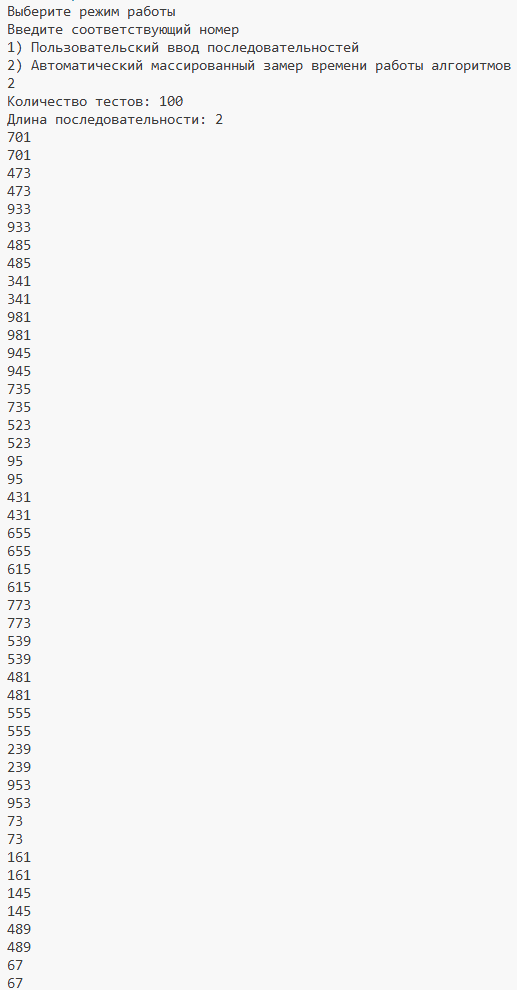
\includegraphics[width = 0.7\textwidth]{example_4.png}
		\captionof{figure}{Начало}
		\label{fig:4}
	\end{center}
		\begin{center}
		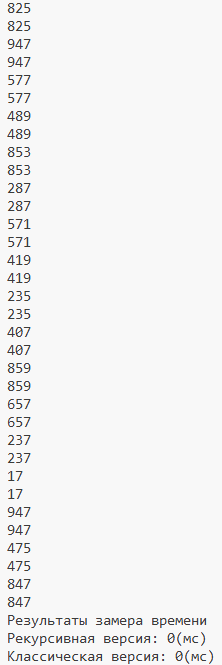
\includegraphics[width = 0.4\textwidth]{example_5.png}
		\captionof{figure}{Окончание}
		\label{fig:5}
	\end{center}
	\subsection{Вывод} 
	Была выполнена программная реализация двух режимов взаимодействия. Также были приведены результаты запуска программной реализации этого режима со всеми возможными исходами.
		\newpage
	\section{Исследовательская часть}
	\subsection{Цель}
	Сделать теоретическую оценку трудоемкости каждого из алгоритмов и провести сравнение с результатами работы программной реализации, а также теоретическую оценку памяти каждого из алгоритмов.
	\subsection{Оценка затрачиваемой памяти алгоритмов}
	Для рекурсивной реализации каждый раз инициализируется одна целочисленная переменная. Однако, глубина вызова рекурсии равна n(где n --- длина числовой последовательности). Таким образом, асимптотика по памяти для рекурсивной реализации будет $O(n)$, причем асимптотика для каждого отдельного вызова --- $O(1)$.\par
	В итеративной реализации единожды инициализируется целочисленная переменная. После чего в цикле больше не происходит инициализаций. Таким образом, асимптотика по памяти для итеративной реализации будет $O(1)$.
	\subsection{Оценка трудоемкости алгоритмов}
	
	Модель оценки в условных единицах:\par
	1) операции стоимостью 1 --- >(проверка: больше ли),==(проверка на равенство);\par
	2) операции стоимостью 2 --- \%(нахождение остатка при делении);\par
	Рассмотрим трудоемкость алгоритмов для последовательности длины n. Для обоих алгоритмов она будет одинаково вычисляться.\par
	\textbf{Рекурсивный и итеративный алгоритм}\par
	Если номер члена последовательности меньше n: $C = 1+3$.\par
	Если номер члена последовательности равен n: $C = 1$.\par
	Таким образом общая теоретическая оценка трудоемкости для обоих алгоритмов будет описываться таким рекуррентным соотношением: $F(n) = F(n-1) + C = n\cdot C$(где C --- константа).
	
	\newpage
	На рисунке ~\ref{fig:6} представлен график зависимости времени работы каждого из алгоритмов относительно длины последовательности.
	\begin{center}
		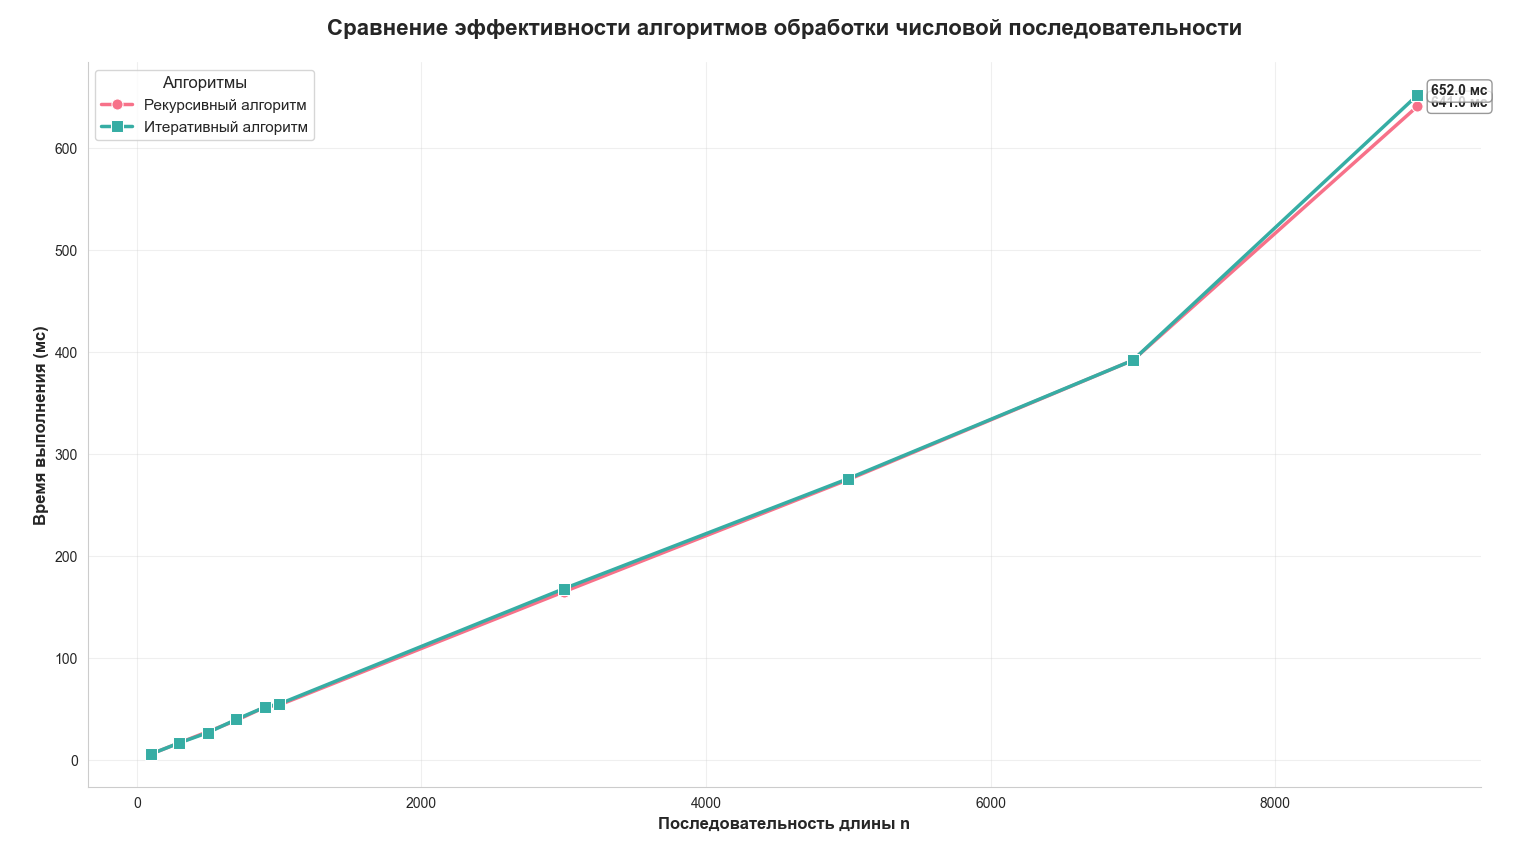
\includegraphics[width = 0.7\textwidth]{graphic.png}
		\captionof{figure}{График}
		\label{fig:6}
	\end{center}
	\subsection{Вывод} 
	По теоретическим оценкам оба алгоритма одинаково оптимальны по времени. По результатам замеров времени чуть медленнее работает итеративная реализация. После же анализа затрат памяти было выявлено, что рекурсивная реализация затрачивает гораздо больше ресурсов.
	\newpage
	\begin{center}
		\section*{ЗАКЛЮЧЕНИЕ}
		\addcontentsline{toc}{section}{ЗАКЛЮЧЕНИЕ}
	\end{center}
	
	В результате выполнения лабораторной работы была достигнута цель работы, заключавшаяся в проведении сравнительного анализа рекурсивного и нерекурсивного алгоритмов.\par
	Также были выполнены все задачи:\par
	1) разработать рекурсивный и нерекурсивный алгоритмы решения задачи, согласно варианту;\par
	2) описаны средства разработки и инструменты замера процессорного времени выполнения реализации алгоритмов;\par
	3) реализованы разработанные алгоритмы;\par
	4) выполнено тестирование реализации алгоритмов;\par
	5) выполнена теоретическая оценка затрачиваемой реализацией каждого алгоритма памяти(для рекурсивного алгоритма --- на материале анализа высоты дерева рекурсивных вызовов и оценки затрачиваемой на один вызов функции памяти);\par
	6) выполнены замеры процессорного времени выполнения реализации алгоритмов в зависимости от варьируемого входа(одна точка на графике получается делением времени выполнения k идентичных расчетов на k, k >= 100);\par
	7) сделаны выводы из сравнительного анализа реализации рекурсивного и нерекурсивного алгоритмов решения одной и той же задачи, заданной вариантом, по критериям ёмкостной эффективности(на материале теоретической оценки пиковой временной эффективности и на материале результатов измерений).
	\newpage
	\begin{center}
		\section*{СПИСОК ИСПОЛЬЗОВАННЫХ ИСТОЧНИКОВ}
		\addcontentsline{toc}{section}{СПИСОК ИСПОЛЬЗОВАННЫХ ИСТОЧНИКОВ}
	\end{center}
	
	\makeatletter
	\renewcommand{\@biblabel}[1]{#1.}
	\makeatother
	
	\renewcommand{\refname}{}
	\begin{thebibliography}{0}
		\bibitem{lit1} Кормен, Т. Алгоритмы: построение и анализ = Introduction to Algorithms / Т. Кормен, Ч. Лейзерсон, Р. Ривест, К. Штайн ; пер. с англ. под ред. И. В. Красикова. — 3-е изд. — Москва : Вильямс, 2022. — 1328 с. — ISBN 978-5-8459-2087-5.
	\end{thebibliography}
	\newpage
	\begin{center}
		\section*{ПРИЛОЖЕНИЕ А}
		\addcontentsline{toc}{section}{ПРИЛОЖЕНИЕ А}
	\end{center}
	
	В листинге~\ref{list1} приведена программная реализация поставленных задач.
	\begin{flushleft}
		\begin{lstlisting}[label = list1, caption = Программная реализация, language=C++, xleftmargin=0pt, xrightmargin=0pt]
#include <chrono>
#include <iostream>
#include <fstream>
#include <vector>
#include <random>
#include <sstream>

using namespace std;
using namespace chrono;

struct InputError : public exception {
	string message;
	InputError(const string& msg) : message(msg) {}
	const char* what() const noexcept override {
		return message.c_str();
	}
};

struct FileError : public exception {
	string message;
	FileError(const string& msg) : message(msg) {}
	const char* what() const noexcept override {
		return message.c_str();
	}
};

struct IntTypeError : public exception {
	string message;
	IntTypeError(const string& msg) : message(msg) {}
	const char* what() const noexcept override {
		return message.c_str();
	}
};

void recursive() {
	int number;
	cin >> number;
	if (cin.fail()) {
		cin.clear();
		cin.ignore(numeric_limits<streamsize>::max(), '\n');
		throw InputError("Ошибка: неправильный ввод");
	}
	else if (number < 0) {
		throw IntTypeError("Ошибка: введено отрицательное число");
	}
	else if (number > 0) {
		if (number % 2 == 1) {
			cout << number << endl;
		}
		recursive();
	}
}

void classic() {
	int number;
	while (1) {
		cin >> number;
		if (cin.fail()) {
			cin.clear();
			cin.ignore(numeric_limits<streamsize>::max(), '\n');
			throw InputError("Ошибка: неправильный ввод");
		}
		else if (number == 0) {
			break;
		}
		else if (number < 0) {
			throw IntTypeError("Ошибка: введено отрицательное число");
		}
		else if (number % 2 == 1) {
			cout << number << endl;
		}
	}
}

void benchmark() {
	const int NUM_TESTS = 100;
	const int SEQUENCE_LENGTH = 9000;
	
	ofstream file("data.txt", ios::app);
	if (!file.is_open()) {
		throw FileError("Ошибка: не удалось открыть файл");
	}
	
	random_device rand;
	mt19937 generate(rand());
	uniform_int_distribution<int> dist(1, 1000);
	
	vector<long long> recursive_times;
	vector<long long> classic_times;
	
	cout << "Количество тестов: " << NUM_TESTS << endl;
	cout << "Длина последовательности: " << SEQUENCE_LENGTH+1 << endl;
	
	for (int test = 0; test < NUM_TESTS; ++test) {
		vector<int> test_data;
		for (int i = 0; i < SEQUENCE_LENGTH; ++i) {
			test_data.push_back(dist(generate));
		}
		test_data.push_back(0);
		
		{
			auto orig_cin = cin.rdbuf();
			
			stringstream test_stream;
			for (int num : test_data) {
				test_stream << num << " ";
			}
			
			cin.rdbuf(test_stream.rdbuf());
			
			auto start = high_resolution_clock::now();
			recursive();
			auto end = high_resolution_clock::now();
			
			cin.rdbuf(orig_cin);
			
			duration<double, milli> time = end - start;
			recursive_times.push_back(time.count());
		}
		
		{
			auto orig_cin = cin.rdbuf();
			
			stringstream test_stream;
			for (int num : test_data) {
				test_stream << num << " ";
			}
			
			cin.rdbuf(test_stream.rdbuf());
			
			auto start = high_resolution_clock::now();
			classic();
			auto end = high_resolution_clock::now();
			
			cin.rdbuf(orig_cin);
			
			duration<double, milli> time = end - start;
			classic_times.push_back(time.count());
		}
	}
	
	long long recursive_avg = 0, classic_avg = 0;
	for (int i = 0; i < NUM_TESTS; ++i) {
		recursive_avg += recursive_times[i];
		classic_avg += classic_times[i];
	}
	recursive_avg /= NUM_TESTS;
	classic_avg /= NUM_TESTS;
	
	cout << "Результаты замера времени" << endl;
	cout << "Рекурсивная версия: " << recursive_avg << "(мс)" << endl;
	cout << "Классическая версия: " << classic_avg << "(мс)" << endl;
	file << recursive_avg << " " << classic_avg << endl;
}

int main() {
	cout << "Выберите режим работы\n" << "Введите соответствующий номер" << endl;
	cout << "1) Пользовательский ввод последовательностей\n" << "2) Автоматический массированный замер времени работы алгоритмов" << endl;
	
	try {
		int n;
		cin >> n;
		if (n == 1) {
			cout << "Введите последовательность натуральных чисел, завершающуюся 0" << endl;
			
			cout << "Рекурсивная версия:" << endl;
			recursive();
			
			cout << "Введите последовательность еще раз" << endl;
			cout << "Классическая версия:" << endl;
			classic();
		}
		else if (n == 2) {
			benchmark();
		}
		else {
			throw InputError("Ошибка: неправильный ввод");
		}
	}
	catch (const InputError& e) {
		cerr << e.what() << endl;
		return 1;
	}
	catch (const IntTypeError& e) {
		cout << e.what() << endl;
		return 1;
	}
	catch (const exception& e) {
		cerr << "Неизвестная ошибка: " << e.what() << endl;
		return 1;
	}
}
		\end{lstlisting}
	\end{flushleft}
		В листинге~\ref{list2} приведена вспомогательная программная реализация для получения графика зависимости времени работы каждого из алгоритмов относительно длин последовательностей.
	\begin{flushleft}
		\begin{lstlisting}[label = list2, caption = Вспомогательная программная реализация на языке программирования Python, language=Python, xleftmargin=0pt, xrightmargin=0pt]
import pandas as pd
import seaborn as sns
import matplotlib.pyplot as plt
import numpy as np

def graphics(data):
df = pd.DataFrame(data)

df_melted = df.melt(id_vars='sequence_length', 
var_name='Алгоритм', 
value_name='Время (мс)')

sns.set_style("whitegrid")
sns.set_palette("husl", 2)

plt.figure(figsize=(12, 8))

lineplot = sns.lineplot(data=df_melted, 
x='sequence_length', 
y='Время (мс)', 
hue='Алгоритм',
style='Алгоритм',
markers={'Рекурсивный алгоритм': 'o', 'Итеративный алгоритм': 's'},
dashes=False,
markersize=8,
linewidth=2.5)

plt.title('Сравнение эффективности алгоритмов обработки числовой последовательности', 
fontsize=16, fontweight='bold', pad=20)
plt.xlabel('Последовательность длины n', fontsize=12, fontweight='bold')
plt.ylabel('Время выполнения (мс)', fontsize=12, fontweight='bold')

plt.legend(title='Алгоритмы', title_fontsize=12, fontsize=11)

plt.grid(True, alpha=0.3)

last_size = df['sequence_length'].iloc[-1]
for algo in ['Рекурсивный алгоритм', 'Итеративный алгоритм']:
last_point = df[algo].iloc[-1]
plt.annotate(f'{last_point:.1f} мс', 
xy=(last_size, last_point),
xytext=(10, 0), 
textcoords='offset points',
fontsize=10,
fontweight='bold',
bbox=dict(boxstyle="round,pad=0.3", 
facecolor="white", 
alpha=0.8,
edgecolor='gray'))

sns.despine()
plt.tight_layout()

plt.show()

data_1 = {
	'sequence_length': [],
	'Рекурсивный алгоритм': [],
	'Итеративный алгоритм': []
}

with open('data.txt', 'r') as f:
plus = 200
i = 100
while i <= 10**3:
a = f.readline().split()

data_1['sequence_length'].append(i)
data_1['Рекурсивный алгоритм'].append(float(a[0]))
data_1['Итеративный алгоритм'].append(float(a[1]))
i += plus
plus = 2000
i = 1000
while i <= 10**4:
a = f.readline().split()

data_1['sequence_length'].append(i)
data_1['Рекурсивный алгоритм'].append(float(a[0]))
data_1['Итеративный алгоритм'].append(float(a[1]))
i += plus

graphics(data_1)
		\end{lstlisting}
	\end{flushleft}
\end{document}